\documentclass[a4paper,11pt]{article}

\usepackage{ascmac}
\usepackage{amsmath,amssymb}
\usepackage{bm}
\usepackage{graphicx}
\usepackage{url}
\usepackage{booktabs}
\usepackage{array}
\usepackage[margin=25mm]{geometry}
\usepackage{fontspec}
\usepackage{xeCJK}
\setmainfont{Times New Roman}
\setCJKmainfont{Yu Mincho}
\setCJKsansfont{Yu Gothic}
\setCJKmonofont{MS Gothic}
\XeTeXlinebreaklocale "ja"
\XeTeXlinebreakskip=0pt plus 1pt
\setlength{\parindent}{1em}
\renewcommand{\today}{\number\year 年\number\month 月\number\day 日}

\title{Sentence-BERTを用いた用途・予算別PC構成推薦システム}
\author{学籍番号 24026111，氏名 佐藤 信晃}
\date{\today}

\begin{document}
\maketitle

\section{課題設定}

\subsection{背景と解決する問題}
PCを購入する際には，CPU，GPU，メモリ，ストレージ，電源容量など，
多数の部品を用途に応じて選ぶ必要がある。
しかし，初心者が「WQHDでゲームを快適に遊びたい」などの要求を持っていても，
個々の部品名から適切な構成を判断することは難しい。
また，同じ用途でも「動画制作」と「YouTube用の映像編集」のように表現が異なるため，
単純な文字列一致だけでは要求に近い構成を検索できない場合がある。

そこで本課題では，利用者が自然文で入力した用途と予算から，
意味の近いPC構成を推薦するプロトタイプを実装した。
自然文の意味的な近さを扱うため，Sentence-BERT（SBERT）による
文章埋め込みを中核技術として使用する。

一般的なPC販売サイトでは，価格帯や部品名による絞り込みはできるが，
利用者が持つ要求を部品条件へ言い換える作業は利用者自身に委ねられることが多い。
例えば「配信しながらゲームをしたい」という要求から，CPUの並列処理性能，
GPU性能，メモリ容量の優先順位を初心者が決めることは容易ではない。
本システムは，この要求と部品条件の間を，あらかじめ用途説明と結び付けた
PC構成を意味検索することで補う。最終的な購入を自動決定するものではなく，
候補を数件に絞り，比較を始めるための意思決定支援を目的とする。

\subsection{対象ユーザと要求}
対象ユーザは，PC部品について詳しくない学生，ゲーマー，動画制作者などである。
主な要求を以下に示す。

\begin{itemize}
  \item 専門用語を使わず，自然文で用途を入力できる。
  \item 指定した予算を超えない構成だけを比較できる。
  \item 推薦されたCPU，GPU，RAMなどを一覧で確認できる。
  \item 推薦理由と入力文に対する類似度を確認できる。
\end{itemize}

ここで重要なのは，予算を文章の類似度に混ぜず，独立した必須条件として扱う点である。
用途が非常に近くても予算を超える候補を表示すると，推薦として実用性が低い。
そのため，本システムでは最初に予算で候補集合を限定し，その集合内でのみ
意味的な順位を決定する。一方，利用者の好みを完全に把握するには，
ディスプレイ解像度，重視するソフトウェア，静音性などの追加情報も必要になる。
本プロトタイプでは入力を簡潔に保つため，それらを一つの自然文に含める設計とした。

\subsection{想定ユースケース}
利用者はWeb画面に「Apexを高フレームレートで遊びたい」と入力し，
予算を22万円に設定する。
システムは予算内の候補だけを抽出し，入力文と各候補の登録用途との
意味的類似度を計算する。
そして，類似度の高い順にPC構成，概算価格，推薦理由，予算残額を表示する。
例えば，この入力では競技FPS向けの構成が上位になることを期待する。

別の利用場面として，大学生が「レポート作成が中心だが軽いゲームもしたい」と
入力する場合がある。このとき高価なゲーム専用機を提示するのではなく，
予算内で学生向けカテゴリが上位になることが望ましい。また，動画制作者が
「YouTube用の編集とゲームを一台で行いたい」と入力した場合には，
単一用途ではなく複合用途を記述した候補を検索する必要がある。
このように，製品名を直接指定しない複数の表現を同じ検索方式で扱えることを
主要な利用価値とした。


\section{技術概要}

\subsection{Sentence-BERT}
BERTを用いて文の類似度を求める単純な方法では，文の組を一つずつモデルへ
入力する必要があり，多数の候補との比較には計算量が大きい。
Sentence-BERTはSiamese Network構造を用いて，各文を固定長ベクトルへ
変換し，ベクトル間の距離によって文の意味的類似度を高速に計算できるようにした
手法である\cite{SBERT}。

本システムでは，日本語を含む50以上の言語を扱い，文や短い段落を
384次元のベクトルへ写像する
\verb|paraphrase-multilingual-MiniLM-L12-v2|を使用した\cite{ModelCard}。
PC用途の登録文と利用者の入力文は，それぞれ同じ埋め込み空間のベクトルへ
変換される。

\subsection{コサイン類似度}
入力文の埋め込みを$\bm{q}$，候補文の埋め込みを$\bm{d}$とすると，
コサイン類似度は式(\ref{eq:cos})で定義される。

\begin{equation}
  \mathrm{sim}(\bm{q},\bm{d})
  = \frac{\bm{q}\cdot\bm{d}}
  {\|\bm{q}\|_2\|\bm{d}\|_2}
  \label{eq:cos}
\end{equation}

値が大きい候補ほど，入力文と意味的に近いと判断する。
実装では埋め込み生成時にL2正規化を行った後，
\verb|sentence_transformers.util.cos_sim|を用いて類似度を計算した。
Sentence Transformersの公式文書でも，文埋め込み同士の意味的類似度の
算出方法としてコサイン類似度が示されている\cite{STSDoc}。

L2正規化後のベクトルでは各ベクトルのノルムが1となるため，
コサイン類似度は内積と等価になる。本実装ではライブラリ関数を使用しているが，
順位付けの考え方は，入力ベクトルが指す方向と候補ベクトルが指す方向の近さを
比較するものである。ベクトルの大きさではなく方向を見るため，
文の長さが多少異なる候補も比較できる。ただし，類似度は性能の達成度や
購入後の満足度を直接表す確率ではない。例えば0.8という値を
「80\%満足する」と解釈することはできず，同じ候補集合内の相対的な
順位付けに用いる指標である。

\subsection{キーワード検索との違い}
キーワード検索では，入力文と登録文が共有する語を数えることで候補を探せる。
実装が単純で結果も説明しやすい反面，「映像を作りたい」と「動画編集」のように
共通語が少ない言い換えを見落とす可能性がある。SBERTは文全体をベクトル化するため，
表面的な文字列が一致しなくても，学習済みモデルが捉えた意味の近さを利用できる。
PC用途では，ゲーム名，解像度，制作作業など多様な表現が入力されるため，
この性質が適していると考えた。

一方，数値や固有名詞の厳密な一致は意味検索だけでは保証されない。
「16GB以上」や「30万円以内」のような条件は，文章に埋め込んで比較するより，
構造化した列に対する数値判定の方が確実である。本設計が予算をフィルタ，
用途をSBERTという二種類の処理に分けたのは，柔軟な条件と厳密な条件を
それぞれ適切な方法で扱うためである。

\subsection{推薦用コーパス}
推薦用コーパスはCSV形式で独自に作成した26件のPC構成である。
各行は用途文，概算価格，CPU，GPU，RAM，SSD，電源，カテゴリ，
推薦理由を持つ。
ゲーム，配信，動画編集，3D制作，画像生成AI，機械学習，学生向けなど，
異なる目的を含めた。

各用途文は，単に部品名を並べるのではなく，「誰が何をどの程度行いたいか」が
分かる一文として記述した。カテゴリは評価時の正解ラベルとして用い，
推薦理由は検索後に人が候補を確認するための説明として用いる。
埋め込みの計算対象は\verb|use_case|列だけであり，カテゴリ名や推薦理由を
入力ベクトルとの比較へ含めていない。評価ラベルを検索文へ混入させず，
用途説明の意味だけから順位を決めるためである。

26件という規模は実サービスには小さいが，プロトタイプでは候補文を目視確認でき，
誤推薦の理由を一件ずつ分析できる利点がある。また，同じ「ゲーム」でも
競技FPS，WQHD，4K，VR，配信併用などを分け，近接しやすい候補を意図的に含めた。
これにより，全く異なる用途を区別するだけでなく，類似した用途間の順位も
観察できるようにした。

本プロトタイプの目的は市場価格を厳密に見積もることではなく，
文章埋め込みによる意味検索の動作を検証することである。
したがって，価格と部品構成は固定した検証用データであり，
実店舗の在庫や価格を外部APIから取得していない。

コーパスに含まれる26件の概算価格帯を図\ref{fig:corpus-price}に示す。
候補は10万円台から60万円台まで存在し，特に20万円台と30万円台を
中心に構成されている。これは，中価格帯のゲーム，配信，制作用途を
複数比較できるようにしたためである。一方，50万円以上の候補は少なく，
高価格帯では用途の違いを細かく比較しにくいというデータ上の偏りがある。

\begin{figure}[htbp]
  \centering
  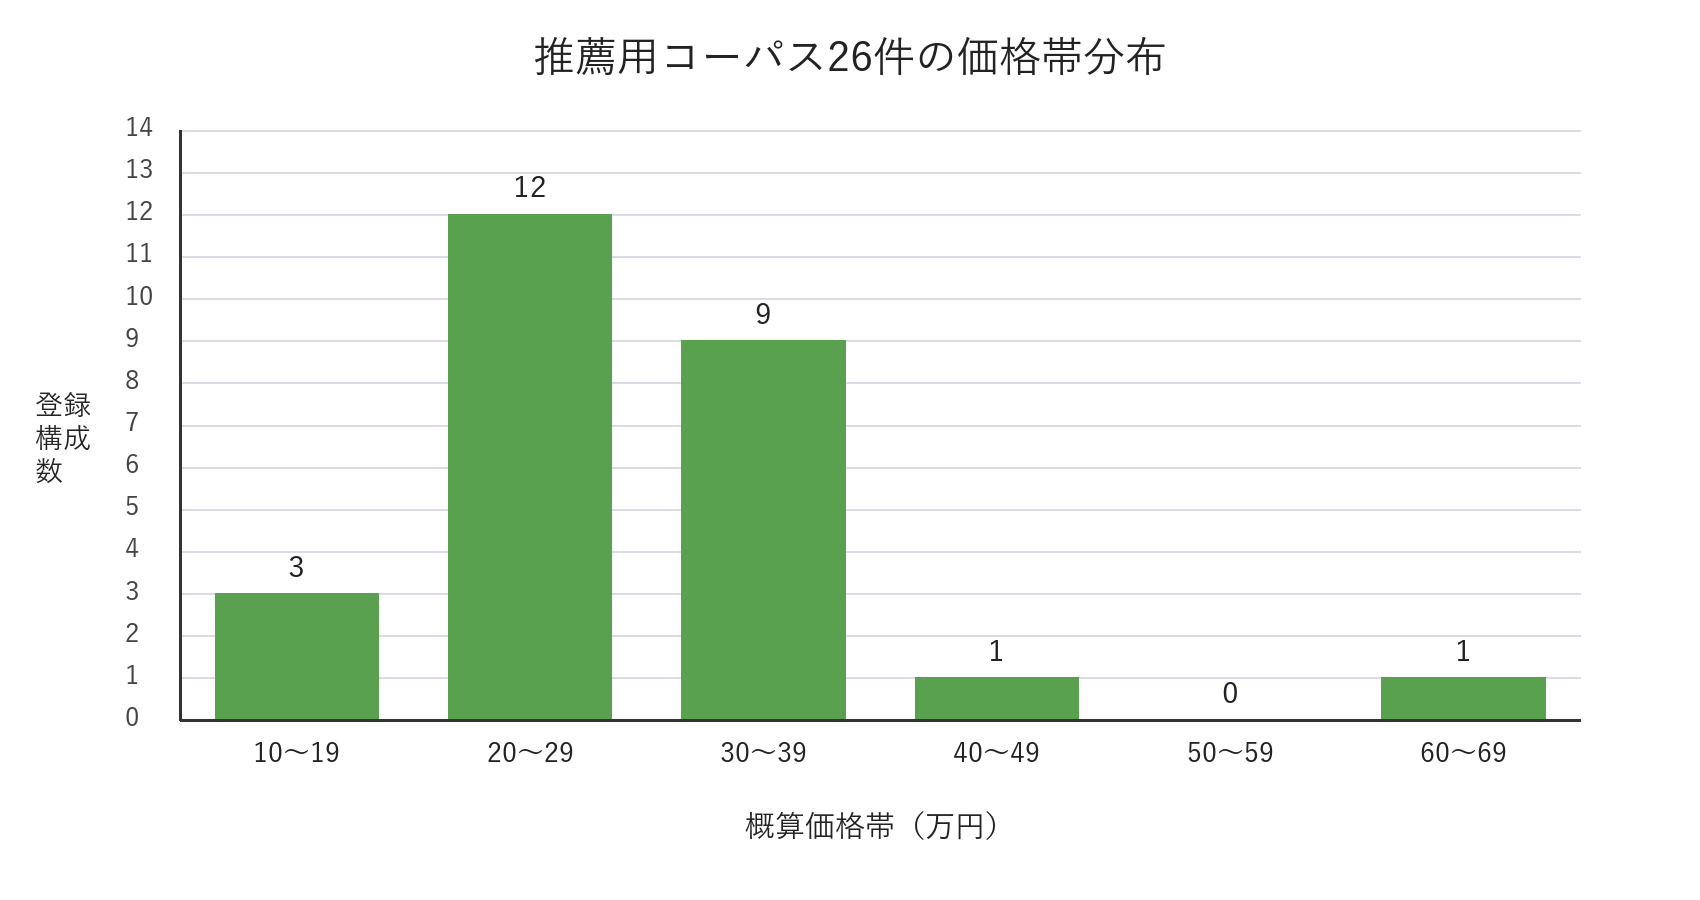
\includegraphics[width=0.78\textwidth]{figures/corpus_price_distribution.png}
  \caption{推薦用コーパス26件の価格帯分布}
  \label{fig:corpus-price}
\end{figure}


\section{システムの設計}

\subsection{入出力}
入力は用途を表す自然文，予算，表示候補数の三つである。
予算は14万円から60万円，候補数は1件，3件，5件から指定できる。
出力は類似度順のPC構成であり，各候補についてカテゴリ，登録用途，
CPU，GPU，RAM，SSD，電源，概算価格，推薦理由，予算残額を表示する。

入力文は自由記述とし，語数や定型句を要求しない。ただし，空文字では意味検索が
成立しないため検索を実行しない。予算の下限を14万円としたのは，
コーパス中の最安構成と対応させ，通常の画面操作で必ず一件以上の候補が
残るようにするためである。候補数を1，3，5件に限定したのは，
一件だけを素早く確認する利用と，複数案を比較する利用の両方を想定しつつ，
情報過多を避けるためである。

\subsection{処理フロー}
システム全体の処理フローを図\ref{fig:flow}に示す。

\begin{figure}[htbp]
  \centering
  \setlength{\fboxsep}{6pt}
  \begin{tabular}{c}
    \fbox{利用者が用途文・予算・候補数を入力}\\
    $\downarrow$\\
    \fbox{CSVを読み込み，予算以下の候補を抽出}\\
    $\downarrow$\\
    \fbox{SBERTで入力文を384次元ベクトルへ変換}\\
    $\downarrow$\\
    \fbox{候補ベクトルとのコサイン類似度を計算}\\
    $\downarrow$\\
    \fbox{上位$k$件のPC構成と推薦理由を表示}
  \end{tabular}
  \caption{PC構成推薦システムの処理フロー}
  \label{fig:flow}
\end{figure}

図\ref{fig:flow}の各段階は，条件による抽出と意味による並べ替えに大別できる。
最初の予算抽出で候補の行番号を保存し，その行に対応する埋め込みだけを
類似度計算へ渡す。これにより，予算外の候補が高い類似度を得ても結果には入らない。
その後，得点の上位から指定件数を選び，元のCSV行と結合して画面表示用の
辞書を作る。意味検索の結果と部品情報を同じ行番号で結び付けるため，
類似度と異なる構成が表示されないようにしている。

\subsection{モジュール構成}
プロトタイプはPythonとStreamlitで実装した。
主な関数を表\ref{tab:functions}に示す。

\begin{table}[htbp]
  \centering
  \caption{主な関数と役割}
  \label{tab:functions}
  \begin{tabular}{ll}
    \toprule
    関数 & 役割\\
    \midrule
    \verb|load_data| & CSVの読込みと必須列の検証\\
    \verb|load_model| & Sentence-BERTモデルの読込み\\
    \verb|load_corpus_embeddings| & 全候補文の事前ベクトル化\\
    \verb|recommend| & 予算抽出，類似度計算，上位候補の生成\\
    \verb|evaluate| & 固定した10件によるTop-$k$評価\\
    \bottomrule
  \end{tabular}
\end{table}

モジュール間では，データ読込み，モデル処理，推薦ロジック，画面表示を分離した。
特に\verb|recommend|はStreamlitの部品へ直接依存せず，入力値から
推薦結果のリストを返す。そのため，同じ処理を検索画面と一括評価の両方から
再利用できる。評価だけ別の推薦処理を実装すると，本番画面と異なる条件を
測定する危険があるため，共通関数を用いる構成とした。

\subsection{キャッシュ設計}
モデルの読込みと全文の埋め込み計算を検索のたびに行うと応答が遅くなる。
そこで，モデルとコーパス埋め込みには
\verb|st.cache_resource|を適用した。
CSV読込みには\verb|st.cache_data|を適用した。
初回検索ではモデル読込みが必要だが，2回目以降は入力文だけを
ベクトル化すればよい。

キャッシュは応答性を改善する一方，CSVを変更した際に古いデータや埋め込みが
残る可能性がある。本プロトタイプでは開発中にStreamlitのキャッシュを
消去することで対応する。実運用では，ファイルの更新日時やデータのハッシュ値を
キャッシュキーへ含め，CSVと埋め込みの対応を保証する必要がある。


\section{プロトタイプの実装}

\subsection{推薦処理}
推薦処理では，最初に空文字，予算，候補数を検証する。
次に，CSVの全候補から概算価格が予算以下の行番号だけを取得する。
入力文を正規化済みベクトルに変換し，対象候補のベクトルとの
コサイン類似度を一括計算する。
最後に\verb|topk|で上位候補を選び，類似度と予算残額を付加して返す。
中核部分を以下に示す。

\begin{screen}
\begin{verbatim}
query_embedding = model.encode(
    query,
    convert_to_tensor=True,
    normalize_embeddings=True,
)
eligible_embeddings = corpus_embeddings[eligible_indices]
scores = util.cos_sim(query_embedding,
                      eligible_embeddings)[0]
top = scores.topk(k=min(top_k, len(eligible_indices)))
\end{verbatim}
\end{screen}

\verb|min|を用いるのは，予算内候補が指定件数より少ない場合にも
\verb|topk|が範囲外エラーにならないようにするためである。
また，検索後には概算価格を予算から引いて残額を計算する。
残額は順位には使わないため，安い候補が自動的に上位になるわけではない。
本システムにおける順位の第一基準は用途の類似度であり，
予算は可否を決める条件である。この役割分担により，
「予算を使い切る構成」と「安価で余裕を残す構成」を上位候補間で比較できる。

\subsection{ユーザインタフェース}
画面は「構成を検索」と「性能評価」の二つのタブで構成した。
検索タブでは，自然文入力，予算スライダー，候補数選択を一つの画面に配置した。
結果は候補ごとの枠に分け，部品名と概算価格を表示する。
類似度だけでなく，登録用途と推薦理由も表示することで，
利用者が推薦結果を解釈しやすいようにした。

類似度だけを表示した場合，利用者はなぜその構成が選ばれたか判断しにくい。
そこで登録用途を併記し，入力文とどの点が近いかを利用者自身が確認できるようにした。
推薦理由は，部品の役割を短文で補足する情報であり，類似度から自動生成した文章ではない。
あらかじめCSVへ登録した説明を表示するため，同じ候補には常に同じ説明が示され，
結果の再現性を保てる。

性能評価タブでは，ボタン一つで10件を評価し，Top-1正解率，
Top-3正解率，各入力の期待カテゴリと予測カテゴリを表示する。
これにより，推薦結果を目視するだけでなく，同じ条件で繰り返し比較できる。

\subsection{実行結果の例}
用途文に「モンハンをWQHDの高画質かつ快適に遊びたい」，
予算に30万円，表示候補数に3件を指定した実行画面を
図\ref{fig:recommendation-result}に示す。
画面上では，入力欄と検索条件に続けて，類似度が最も高い候補の
部品構成，概算価格，推薦理由，予算残額が一つのカードにまとめられている。

\begin{figure}[htbp]
  \centering
  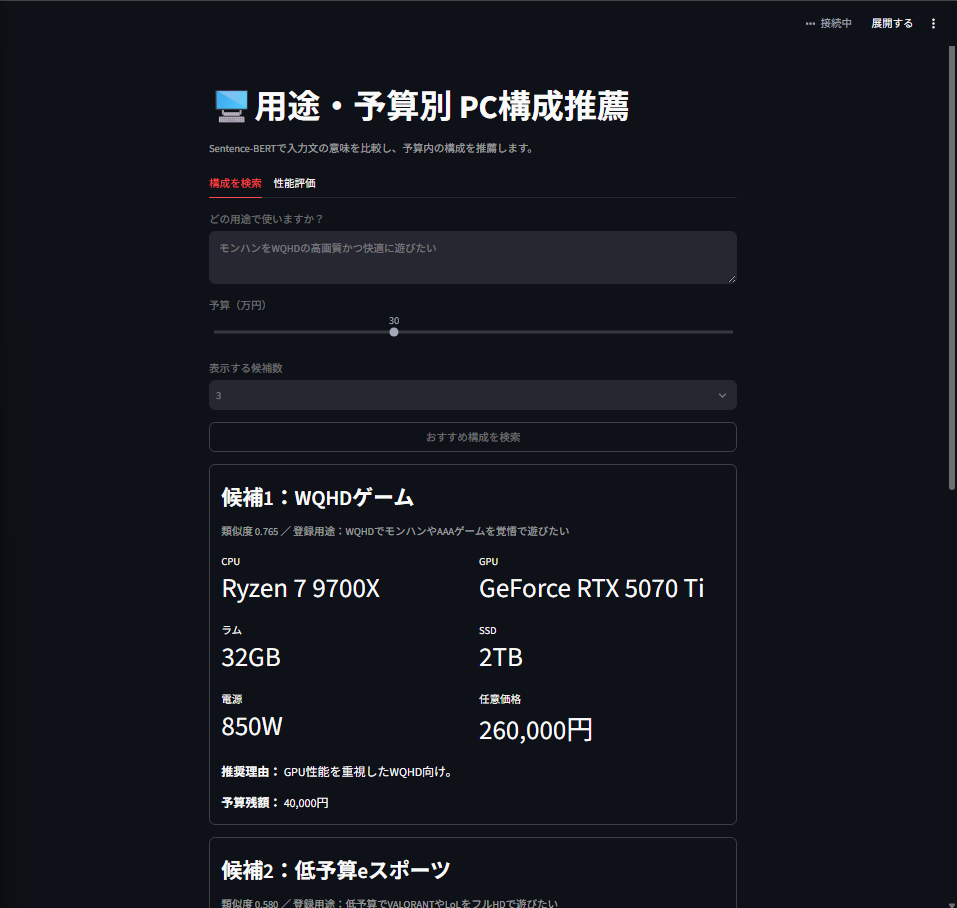
\includegraphics[width=0.82\textwidth]{figures/recommendation_result.png}
  \caption{PC構成推薦の実行画面（入力条件と第1候補）}
  \label{fig:recommendation-result}
\end{figure}

図\ref{fig:recommendation-result-continued}は同じ検索結果の続きであり，
第2候補と第3候補の構成を示している。
利用者は画面をスクロールすることで，上位候補の部品構成と価格を
同じ形式で比較できる。

\begin{figure}[htbp]
  \centering
  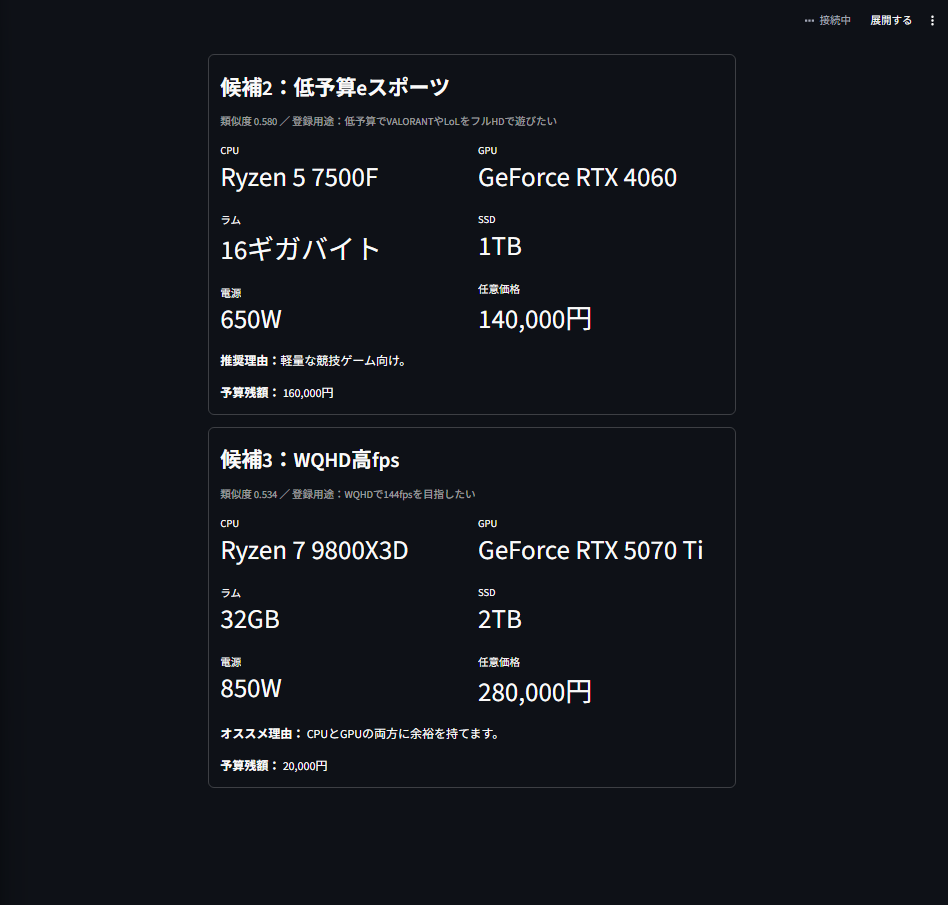
\includegraphics[width=0.82\textwidth]
    {figures/recommendation_result_continued.png}
  \caption{PC構成推薦の実行画面（第2候補と第3候補）}
  \label{fig:recommendation-result-continued}
\end{figure}

このときの上位3候補を表\ref{tab:recommendation-example}に示す。
1位は「WQHDゲーム」で，類似度は0.765であった。
入力文に含まれる「モンハン」，「WQHD」，「高画質」という特徴が，
登録用途の「WQHDでモンハンやAAAゲームを高画質で遊びたい」と
意味的に強く対応した結果である。

\begin{table}[htbp]
  \centering
  \caption{実行画面における上位3候補}
  \label{tab:recommendation-example}
  \begin{tabular}{clclrr}
    \toprule
    順位 & カテゴリ & 類似度 & 主な構成 & 価格 & 予算残額\\
    \midrule
    1 & WQHDゲーム & 0.765 & Ryzen 7 9700X / RTX 5070 Ti
      & 260,000円 & 40,000円\\
    2 & 低予算eスポーツ & 0.580 & Ryzen 5 7500F / RTX 4060
      & 140,000円 & 160,000円\\
    3 & WQHD高fps & 0.534 & Ryzen 7 9800X3D / RTX 5070 Ti
      & 280,000円 & 20,000円\\
    \bottomrule
  \end{tabular}
\end{table}

1位の候補は用途との対応が明確であり，予算条件も満たした。
一方，2位には「低予算eスポーツ」が選ばれた。
これはゲーム用途という共通性を捉えたものの，WQHD高画質という要求への
適合度は低い。3位の「WQHD高fps」は解像度の要求には合うが，
高画質よりフレームレートを重視する登録文であるため，1位より低くなった。
この例から，SBERTは用途の意味を反映して順位付けできる一方，
類似度だけでは画質，解像度，フレームレートなどの個別条件を
常に厳密に制約できるわけではないことが分かる。

\subsection{評価方法}
CSVの用途文をそのまま入力すると評価が過度に容易になるため，
意味を保った言い換え文を10件用意した。
各入力には，正解と期待するカテゴリと，そのカテゴリの構成が含まれる予算を設定した。

評価指標はTop-1正解率とTop-3正解率である。
テスト数を$N$，正解カテゴリを$y_i$，上位$k$件のカテゴリ集合を
$P_i^{(k)}$とすると，Top-$k$正解率を式(\ref{eq:topk})で求める。

\begin{equation}
  \mathrm{Accuracy@}k =
  \frac{1}{N}\sum_{i=1}^{N}
  \mathbf{1}\left[y_i \in P_i^{(k)}\right]
  \label{eq:topk}
\end{equation}

Top-1は最初に提示される候補の正確さを表し，利用者が一件だけ確認する場面に対応する。
Top-3は比較候補まで含めて目的のカテゴリを発見できる割合であり，
推薦システムとしての候補抽出能力を表す。各テストでは期待カテゴリの価格以上の
予算を設定し，正解候補が予算フィルタで除外されない条件にした。
したがって本評価は，価格設定の妥当性ではなく，予算内に存在する正解を
意味検索で上位へ並べられるかを確認するものである。

比較可能性を持たせるため，全テストに同一モデル，同一コーパス，同一の
候補数3件を使用した。ただし，10件はカテゴリごとに一件ずつ無作為抽出した
標本ではなく，代表的な利用場面を選んだ機能検証用データである。
このため正解率に信頼区間を付けて一般化性能を主張するのではなく，
想定した代表入力で機能が成立するかを確認する評価として位置付ける。

\subsection{評価結果}
評価結果を表\ref{tab:result}に示す。

\begin{table}[htbp]
  \centering
  \caption{言い換え入力10件に対する評価結果}
  \label{tab:result}
  \begin{tabular}{lcc}
    \toprule
    指標 & 正解数 & 正解率\\
    \midrule
    Top-1 & 10/10 & 100.0\%\\
    Top-3 & 10/10 & 100.0\%\\
    \bottomrule
  \end{tabular}
\end{table}

例えば「WQHDでゲームを快適に遊びたい」，予算28万円という入力に対し，
1位は「WQHDゲーム」で，コサイン類似度は0.883であった。
2位は「競技FPS」で0.741，3位は「低予算eスポーツ」で0.634であり，
用途の意味に対応した順位となった。

全10件で正解したことから，今回用意した用途の範囲では，
登録文と完全一致しない入力でも意味的に近い構成を取得できた。
一方，評価データは開発者が作成した10件のみであり，
未知の利用者による評価ではない。
したがって，100\%という値を一般的な推薦性能として解釈することはできない。

各入力における1位候補の類似度を図\ref{fig:evaluation-similarity}に示す。
10件の値は0.580から0.931の範囲であり，全件正解であっても
入力によって確信度に差があることが分かる。VRゲームは0.931，
WQHDゲームは0.910と高かった一方，競技FPSは0.580，
3D制作は0.687にとどまった。したがって，カテゴリ一致率だけでなく，
類似度の分布も併せて確認することで，表現の追加が必要な用途を発見できる。

\begin{figure}[htbp]
  \centering
  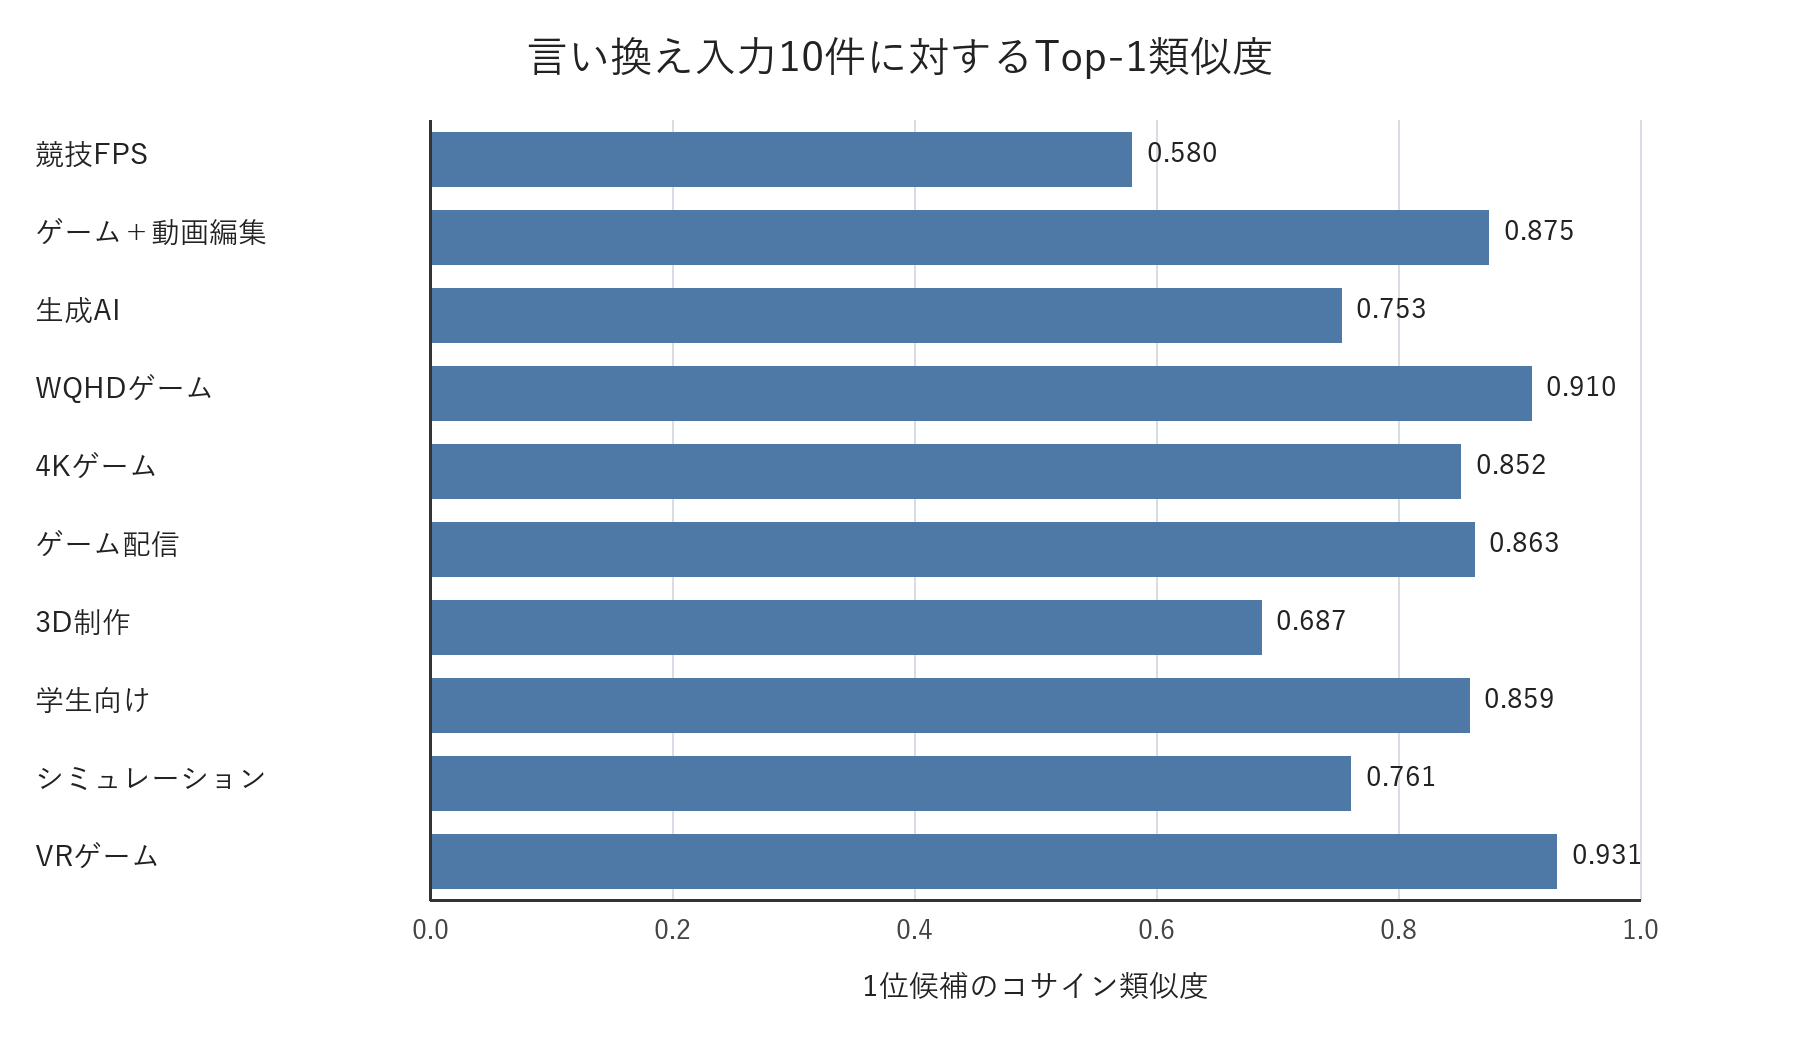
\includegraphics[width=0.88\textwidth]{figures/evaluation_similarity.png}
  \caption{言い換え入力10件に対するTop-1類似度}
  \label{fig:evaluation-similarity}
\end{figure}

また，Top-1とTop-3が同じ100\%であったため，今回の10件だけでは
候補数を増やす効果を比較できなかった。これはシステムが完全であることを意味せず，
評価例が既存カテゴリと明確に対応していた可能性が高い。
実際の利用では，「安くて静かでAIも少し試したい」のような複合的で曖昧な文，
誤字を含む文，コーパスに存在しないソフトウェア名が入力される。
次の評価では，このような難易度別の入力群を用意し，Top-1とTop-3の差，
類似度の分布，予算変更による順位変化を比較する必要がある。


\section{最終的なシステムの考察}

\subsection{期待される成果}
完成形では，利用者が部品名を知らなくても，用途と予算だけで
比較の出発点となるPC構成を得られる。
キーワード一致ではなく文章埋め込みを使用するため，
「動画編集」と「YouTube用の映像制作」のような言い換えにも対応できる。
また，外部の生成AI APIに依存せず，ローカルで同じ入力に対して
再現可能な類似度を計算できる。

販売員へ相談する前の自己整理や，複数の完成品PCを比較する際の基準作りにも利用できる。
利用者は推薦された部品を絶対的な正解として受け取るのではなく，
登録用途と推薦理由を読み，自分の要求に近い点と不足する点を確認できる。
管理者側は新しい用途や価格帯の構成をCSVへ追加することで，
モデルを再学習せずに検索対象を更新できる。これは，少量の候補データから
運用を開始し，利用記録を見ながら段階的に拡充する場合に有効である。

\subsection{問題点}
第一に，コーパスが26件と小さく，候補に存在しない用途や複合的な要求には弱い。
類似度は文章同士の意味の近さを表すが，PC部品間の互換性や，
実際のフレームレートを保証する値ではない。

第二に，価格を固定値としているため，市場価格の変動や在庫を反映できない。
また，「静音」「省電力」などを入力しても，候補文の情報だけで順位が決まり，
消費電力や騒音の実測値を用いた制約判定は行っていない。

第三に，評価用入力と期待カテゴリを開発者が作成している。
同じ人物がコーパスと評価データを作ることで，表現やカテゴリに偏りが入る。
実利用者が自由に入力する場合の誤記，長文，曖昧な要求については
追加検証が必要である。

第四に，評価指標がカテゴリ一致だけであり，部品構成の品質や画面の使いやすさを
直接測っていない。期待カテゴリが一致しても，予算残額が大きすぎる，
特定ソフトウェアの推奨要件を満たさないなど，利用者にとって不十分な場合がある。
逆に，期待カテゴリとは異なっても，部品構成としては要求を満たす候補もあり得る。
したがってカテゴリ一致率は検索機能の一側面であり，
推薦全体の品質を表す唯一の指標ではない。

\subsection{改善案}
今後は用途文と構成を増やし，複数人が作成した評価データを
訓練・調整用と最終評価用に分離する。
価格，消費電力，GPUメモリ，筐体サイズなどは文章類似度とは別の
構造化条件として扱う。
類似度が低い場合には無理に推薦せず，追加質問や「該当候補なし」を
提示する閾値も必要である。

さらに，SBERTによる検索結果を第一段階の候補抽出とし，
第二段階で部品互換性と定量条件を規則ベースで検証する構成が考えられる。
この二段階構成により，文章の柔軟な検索能力と，PC構成に必要な
厳密な制約判定を両立できる。

評価方法については，コーパス作成者とは別の協力者に入力文と妥当な候補を
作成してもらい，少なくとも各カテゴリに複数例を用意する。
さらに，検索成功率だけでなく，推薦理由の分かりやすさ，候補比較に要した時間，
最終候補への納得度を5段階で回答してもらうユーザビリティ評価を組み合わせる。
定量条件については，例えば解像度，目標フレームレート，必要GPUメモリを
個別項目として収集し，SBERTの得点と制約充足率を別々に表示する。

類似度の閾値は固定値を恣意的に決めるのではなく，正解例と不正解例の
スコア分布を評価データから求めて設定することが望ましい。
閾値未満の場合には追加質問を表示し，「ゲームなら解像度と重視する画質を
入力してください」のように不足情報を補う。これにより，候補が少ないにも
かかわらず最も近い一件を強制的に推薦する問題を抑えられる。

\subsection{まとめ}
本課題では，多言語Sentence-BERTを用いて，利用者の用途文と
PC構成の登録用途を384次元の文章埋め込みへ変換し，
コサイン類似度と予算条件から候補を推薦するプロトタイプを実装した。
固定した言い換え入力10件ではTop-1，Top-3ともに100\%となり，
小規模な対象範囲で意味検索が機能することを確認した。
今後はコーパスと独立評価データの拡充，価格情報の更新，
部品互換性の検証を追加する必要がある。


\begin{thebibliography}{99}
\bibitem{SBERT}
N. Reimers and I. Gurevych,
``Sentence-BERT: Sentence Embeddings using Siamese BERT-Networks,''
Proceedings of EMNLP-IJCNLP 2019, pp.~3982--3992, 2019.
\url{https://arxiv.org/abs/1908.10084}

\bibitem{ModelCard}
Sentence Transformers,
``paraphrase-multilingual-MiniLM-L12-v2 Model Card,''
\url{https://huggingface.co/sentence-transformers/paraphrase-multilingual-MiniLM-L12-v2},
閲覧日：2026年7月25日.

\bibitem{STSDoc}
Sentence Transformers,
``Semantic Textual Similarity,''
\url{https://sbert.net/docs/sentence_transformer/usage/semantic_textual_similarity.html},
閲覧日：2026年7月25日.

\bibitem{Streamlit}
Streamlit,
``Streamlit documentation,''
\url{https://docs.streamlit.io/},
閲覧日：2026年7月25日.
\end{thebibliography}

\end{document}
